\documentclass{standalone}
\usepackage{tikz,pgf}
\usetikzlibrary{arrows, decorations.markings}
\begin{document}
	\resizebox{6cm}{6cm}{
	
	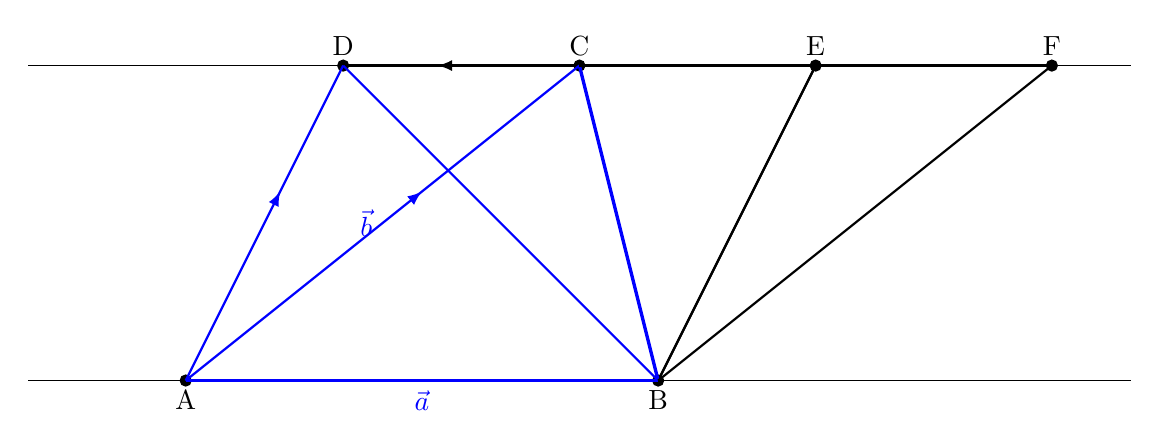
\begin{tikzpicture}[decoration = {markings, mark = at position 0.6 with {\arrow{latex}}
		}]
		\draw (-2,0) -- (12,0);
		\draw (-2,4) -- (12,4);
    	\filldraw[black] (0,0) circle (2pt) node[anchor=north] {A};
		\filldraw[black] (6,0) circle (2pt) node[anchor=north] {B};
		\filldraw[black] (2,4) circle (2pt) node[anchor=south] {D};
		\filldraw[black] (5,4) circle (2pt) node[anchor=south] {C};
		\filldraw[black] (8,4) circle (2pt) node[anchor=south] {E};
		\filldraw[black] (11,4) circle (2pt) node[anchor=south] {F};
	    \draw[blue, thick] (0, 0) -- (6, 0) node[midway, below] {$\vec{a}$};
	    \draw[postaction = decorate, blue, thick] (0, 0) -- (2, 4);
	    \draw[postaction = decorate, black, thick] (5, 4) -- (2, 4);
	    \draw[black, thick] (5, 4) -- (8,4);
	    \draw[black, thick] (6,0) -- (8, 4);
	    \draw[postaction = decorate,blue, thick] (0, 0) -- (5, 4) node[midway, left]{$\vec{b}$};
	    \draw[blue, thick] (6,0) -- (2, 4);
	    \draw[black, thick] (8, 4) -- (6,0);	
	    \draw[blue, very thick] (5, 4) -- (6,0);
	    \draw[black, thick] (11, 4) -- (6, 0);
	    \draw[black, thick] (5,4) -- (11,4);
	\end{tikzpicture}
}
\end{document}